\clearpage
\section{Control Predictivo Adaptativo}
El control Predictivo Adaptativo nace de la necesidad de poder adaptar el control a los cambios propios de un sistema. En procesos industriales reales, la dinámica de una planta rara vez es estática, perturbaciones externas, desgaste de actuadores (como válvulas o bombas) o no linealidades inherentes al proceso provocan que un controlador sintonizado para un punto de operación específico pierda eficiencia al alejarse de este.

El control Predictivo Adaptativo divide el proceso en una parte adaptativa, el cual se encarga de estimar los parámetros del proceso mediante el monitoreo de los esfuerzos de control y las salidas resultantes, y una parte predictiva encargada de tomar la estimación obtenida y generar predicciones del comportamiento del sistema a lo largo de un horizonte predeterminado para luego seleccionar la acción de control que minimice el error futuro proyectado
\subsection{Estimador de Parámetros}
\subsubsection{BATCH LS}
El método de mínimos cuadrados o \textit{BATCH Least Squares} fue utilizado en $1809$ por Carl Friedrich Gauss \cite{stigler1981gauss}, si bien este método fue documentado por varios autores previo a Gauss, este se le atribuye por su uso para determinar la órbita de cuerpos astronómicos.

Este consiste en monitorear $N$ mediciones en una matriz de regresores $M$ y un vector de mediciones $Y$
\[
  \hat{\theta}=(M^TM)^{-1}M^TY
\]

Si bien este enfoque es matemáticamente exacto para procesos offline, resulta inviable para su implementación en sistemas de control en línea, como un PLC industrial. A medida que el proceso avanza, la matriz M crece indefinidamente, saturando la memoria del autómata. Además, el cálculo de la inversa de la matriz $(M^TM)^{-1}$ en cada tiempo de muestreo exige una capacidad de procesamiento computacional que excede los límites prácticos del hardware en tiempo real.

\clearpage
\subsubsection{Recursive Least Squares (RLS)}
Desde la necesidad de implementar algoritmos de indentificación de parámetros en sistemas de control, se propone el método \textbf{RLS} como una adaptación del método presentado anteriormente, cambia el enfoque de BATCH de muestras por un enfoque recursivo, en el cual el estado actual $x_{k}$ se calcula a partir del estado anterior $x_{k-1}$.

\textbf{Filtro Kalman}.


Se asume que el nuevo estado es una combinación lineal del estado anterior y la salida

\[
  \hat{x}_k = W_1\hat{x}_{k-1} + W_2y_k
\]

Tal que la salida es de la forma:
\[
  y_k = C_kx_k + v_k
\]
Donde $C_k$ es la matriz de observación del sensor y $v_k$ es el ruido propio de este.


Luego se exige que el estimador sea \textit{unbiased}, es decir, que en promedio no estime sobre o bajo el valor correcto. Esto puede expresado como la esperanza de la predicción dede ser igual a la esperanza del valor real.

\[
  E[\hat{x}_k] = x_k
\]

Reemplazando se obtiene:
\[
  E[\hat{x}_k] = W_1 E[\hat{x}_{k-1}] + W_2(E[C_k x_k] + E[v_k])
\]
Luego se asume que el ruido del sensor tiene media cero, por lo que $E[v_k]=0$. Junto a esto, se exige que el estimador sea insesgado en todo instante, es decir, $E[\hat{x}_k] = x_k$ y $E[\hat{x}_{k-1}] = x_{k-1}$. Aplicando esto a la ecuación de esperanzas, obtenemos una relación determinista:
\[
  x_k = W_1 x_{k-1} + W_2 C_k x_k
\]
Ahora, como el estimador asume que los parámetros físicos del sistema son constantes en un periodo de muestreo corto, se tiene que $x_k = x_{k-1}$. Factorizando $x_k$ a la derecha:
\[
  x_k = (W_1 + W_2 C_k) x_k
\]
Para que esta igualdad se cumpla para cualquier estado $x_k$, la matriz que lo multiplica debe ser la matriz identidad $I$:
\[
 \therefore W_1 + W_2C_k = I \implies W_1 = I - W_2C_k
\]
Reemplazando $W_1$ en la ecuación del estimador original ($\hat{x}_k = W_1\hat{x}_{k-1} + W_2y_k$), manteniendo el orden matricial correcto:
\[
  \hat{x}_k = (I - W_2C_k)\hat{x}_{k-1} + W_2y_k
\]
Multiplicando y reordenando:
\[
  \hat{x}_k = \hat{x}_{k-1} - W_2C_k\hat{x}_{k-1} + W_2y_k
\]
Así finalmente se factoriza $W_2$ (al cual llamaremos $K$, la ganancia de Kalman) para obtener la expresión de predictor-corrector:
\begin{equation}
  \hat{x}_k = \hat{x}_{k-1} + K(y_k - C_k\hat{x}_{k-1})
  \label{kalman}
\end{equation}

El filtro de Kalman es una generalización del método RLS, útil para estimar estados de un sistema. Desde esta expresión es posible derivar el estimador de parámetros RLS

\textbf{Mínimos cuadrados}

Primero se define el error como la diferencia en el vector de mediciones $Y$ y la salida del modelo $\hat{Y} = \phi \theta$, donde $\phi$ contiene las entradas y salidas medidas y $\theta$ contiene los parámetros desconocidos
\[
  E = Y - \phi \theta
\]

De esta expresión se define la función de costos como los mínimos cuadrados, esto es necesario debido a que el algoritmo sólo evalúa el error como un escalar. Por lo que si se utilizara suma simple de componentes, el error sería gravemente subestimado.

Por ejemplo se propone el siguiente vector de error:
\[
  E = \begin{bmatrix} 5 & -3 & -2 \end{bmatrix}^T
\]
Si se sumaran todos sus componentes el error visto por el algoritmo sería $5 - 3 - 2 = 0$, en cambio utilizando los mínimos cuadrados:
\[
  J(\theta) = E^T E = \begin{bmatrix} 5 & -3 & -2 \end{bmatrix} \begin{bmatrix} 5 \\ -3 \\ -2 \end{bmatrix} = 38
\]

Es así que la función de costos del error se define como

\[
  J(\theta) = E^T E
\]


\[
  J(\theta) = (Y - \phi \theta)^T (Y - \phi \theta)
\]

\[
  J(\theta) = (Y^T - \theta^T \phi^T) (Y - \phi \theta)
\]

\[
  J(\theta) = Y^TY - Y^T\phi\theta - \theta^T \phi^T Y + (\theta^T \phi^T)(\phi \theta)
\]

\begin{equation}
  J(\theta) = Y^TY - 2\theta^T\phi^TY + \theta^T \phi^T \phi \theta
  \label{costos}
\end{equation}

Luego, es de interés minimizar el error, asegurando que el modelo se acerca lo más posible a las mediciones reales. Para esto se toma el jacobiano (derivada matricial) de la ecuación \ref{costos} con respecto al vector $\theta$ y se iguala a cero:

\[
  \frac{\partial J}{\partial \theta} = 0 - 2\phi^TY + 2\phi^T\phi\theta = 0
\]

Despejando $\theta$ se obtiene
\[
  2\phi^T\phi\theta = 2\phi^TY
\]

\begin{equation}
  \theta = (\phi^T\phi)^{-1}\phi^TY
  \label{gaussnormal}
\end{equation}

Esta ecuación es conocida como la ecuación normal de Gauss, si se generaliza a instantes $k$ queda como

\[
  \hat{\theta}_k = (\sum_{i=1}^{k} \phi_i\phi^T_i)^{-1} (\sum_{i=1}^{k} \phi_i y_i) 
\]

Luego, se define al término que acumula información como la matriz de covarianza del sistema, también conocida como la matriz de información de Fisher. 

\[
  P_k = (\sum_{i=1}^{k} \phi_i\phi^T_i)^{-1}
\]

Reescribiendo el Batch se tiene

\[
  \hat{\theta}_k = P_k (\sum_{i=1}^{k} \phi_i y_i) 
\]

Ahora, como se menciona al inicio de esta sección, en sistemas de control es muy costoso implementar esta forma de cálculo debido a la cantidad de muestras y necesidad de invertir una matriz. Es por esto que se debe aplicar una estructura recursiva al algoritmo implementado


\[
  P_k^{-1} = (\sum_{i=1}^{k-1} \phi_i\phi^T_i + \phi_k\phi_k^T)
\]

\[
  P_k^{-1} = (P_{k-1}^{-1} + \phi_k\phi_k^T)
\]

Ahora que es posible calcular recursivamente la matriz de covarianza, queda solucionar el problema de la matriz inversa, para esto se aplica el lema de inversión de matrices \cite{astrom1995adaptive}        
\begin{equation}
  (A + BCD)^{-1} = A^{-1} - A^{-1}B(C^{-1} + DA^{-1}B)^{-1}DA^{-1}
  \label{lema}
\end{equation}

Según el lema \ref{lema} aplicado al caso de interés $P_k = (P_{k-1}^{-1} + \phi_k \phi_k^T)^{-1} $ se tiene
\begin{itemize}
  \item $A = P_{k-1}^{-1}$
  \item $B = \phi_k$
  \item $C = 1$
  \item $D = \phi_k^T$
\end{itemize}

Luego reemplazando en \ref{lema} se tiene

\[
  (P_{k-1}^{-1} + \phi_k\phi_k^T)^{-1} = P_{k-1} - P_{k-1}\phi_k(1 +  \phi_k^TP_{k-1}\phi_k)^{-1}\phi_k^TP_{k-1}
\]

Luego reemplazando $P_k^{-1} = (P_{k-1}^{-1} + \phi_k\phi_k^T)$ se obtiene

\[
  P_k = P_{k-1} - P_{k-1}\phi_k(1 +  \phi_k^TP_{k-1}\phi_k)^{-1}\phi_k^TP_{k-1}
\]

Luego como el término $(1 +  \phi_k^TP_{k-1}\phi_k)^{-1}$ es simplemente un escalar, el costo computacional disminuye considerablemente.

Ahora, volviendo a la expresión \ref{gaussnormal} se puede escrbir como:

\[
  \hat{\theta}_k = P_k (\sum_{i=1}^{k} \phi_i y_i) 
\]

\[
  P_{k-1}^{-1}\hat{\theta}_{k-1} = (\sum_{i=1}^{k-1} \phi_i y_i) 
\]


\[
  \hat{\theta}_k = P_kP_{k-1}^{-1}\hat{\theta}_{k-1} + P_k\phi_k y_k 
\]

Luego, para simplificar los términos encontrados, primero se aplica el lema expuesto anteriormente \ref{lema}

\[
P_k\phi_k = (P_{k-1} - P_{k-1}\phi_k(1 +  \phi_k^TP_{k-1}\phi_k)^{-1}\phi_k^TP_{k-1})\phi_k
\]

Factorizando por $P_{k-1}\phi_k$ queda

\[
P_k\phi_k = P_{k-1}\phi_k(I - (1 +  \phi_k^TP_{k-1}\phi_k)^{-1}\phi_k^TP_{k-1}\phi_k)
\]


\[
  P_k\phi_k = P_{k-1}\phi_k[I - (1 +  \phi_k^TP_{k-1}\phi_k)^{-1}\phi_k^TP_{k-1}\phi_k]
\]

Ahora aplicando un cambio de variable para poder desarrollar el producto $a = \phi_k^TP_{k-1}\phi_k$

\[
  [1 - (1 + a)^{-1}a] = [1 - \frac{a}{1 + a}] = [\frac{1}{1 + a}]
\]

Volviendo a la ecuación original se tiene

\[
P_k\phi_k = P_{k-1}\phi_k[\frac{1}{1 + \phi_k^TP_{k-1}\phi_k}]
\]

De aquí nace el término $K$, correspondiente al vector de ganancias aplicada a la medición actual.

\[
 K_k = \frac{P_{k-1}\phi_k}{1 + \phi_k^TP_{k-1}\phi_k}
\]

Una vez definido esto, volviendo al lema de inversión

\[
P_k = P_{k-1}
- \underbrace{P_{k-1}\phi_k(1+\phi_k^T P_{k-1}\phi_k)^{-1}}_{K_k}
\phi_k^T P_{k-1}
\]

Luego, como todavía falta definir $P_kP_{k-1}^{-1}$

\[
  P_kP_{k-1}^{-1} = P_{k-1}P_{k-1}^{-1} - K_k\phi_k^T P_{k-1}P_{k-1}^{-1}
\]

Como $P_{k-1}P_{k-1}^{-1} = I$
\[
  P_kP_{k-1}^{-1} = I - K_k\phi_k^T 
\]

Así finalmente


\[
  \hat{\theta}_k = (I - K_k\phi_k^T)\hat{\theta}_{k-1} + K_k y_k 
\]

Luego reordenando, se tiene la misma estructura de la ecuación del filtro de Kalman \ref{kalman} pero para los parámetros del sistema.

\begin{equation}
  \hat{\theta}_k = \hat{\theta}_{k-1} + K_k(y_k - \phi_k^T\hat{\theta}_{k-1}) 
  \label{RLS}
\end{equation}
\[
  \underbrace{\hat{\theta}_k}_{2n \times 1} = 
  \underbrace{
  \begin{bmatrix}
    a_1 \\ a_2 \\ \vdots \\ a_n \\ b_1 \\ b_2 \\ \vdots \\ b_n
  \end{bmatrix}
  }_{2n \times 1}
\]

\[
  \underbrace{\phi^T_k}_{1 \times 2n} = 
  \underbrace{
  \begin{bmatrix}
    -\Delta y_{k-1} & -\Delta y_{k-2} & \dots & \Delta u_{k-1} & \Delta u_{k-2} & \dots
  \end{bmatrix}
  }_{1 \times 2n}
\]
Los valores dentro de $\phi^T_k$ pueden ser valores intantáneos o incrementales dependiendo del tipo de control que se ocupe.

\clearpage
\subsubsection{Adaptación a parámetros variantes: Factor de Olvido ($\lambda$)}

La derivación matemática del algoritmo RLS estándar asume implícitamente que los parámetros del sistema ($\theta$) son constantes en el tiempo. Bajo esta suposición, a medida que el algoritmo acumula más y más datos (aumentando la información de la matriz $\Phi^T\Phi$), la matriz de covarianza $P_k$ decrece de forma monótona, tendiendo a cero ($P_k \to 0$). Físicamente, esto significa que el algoritmo adquiere una "certeza absoluta" sobre su modelo, lo que provoca que el vector de ganancia se anule ($K_k \to 0$). En este punto, el estimador se vuelve ciego e ignora cualquier dato futuro, perdiendo su capacidad de adaptación.

Sin embargo, en procesos industriales reales como la planta de cuatro estanques, cuya dinámica es intrínsecamente no lineal  los parámetros linealizados cambian a medida que el proceso se desplaza a diferentes puntos de operación.

Para evitar que el estimador se vuelva ciego, se introduce una modificación en la función de costo original mediante un \textbf{Factor de Olvido Exponencial ($\lambda$)}. La nueva función de costos asigna mayor peso a los errores recientes:

\[
  J(\theta, k) = \sum_{i=1}^{k} \lambda^{k-i} (y_i - \phi_i^T \theta)^2
\]

Donde $0 < \lambda \le 1$. Típicamente, en aplicaciones industriales, se utilizan valores entre $0.95$ y $0.99$. 

Al aplicar este decaimiento exponencial a la derivación del Lema de Inversión de Matrices, las ecuaciones de actualización del RLS se modifican ligeramente. La actualización de los parámetros ($\hat{\theta}_k$) mantiene su estructura original, pero las ecuaciones de la ganancia ($K_k$) y de la matriz de covarianza ($P_k$) quedan definidas de la siguiente forma:

\begin{equation}
  K_k = \frac{P_{k-1}\phi_k}{\lambda + \phi_k^T P_{k-1} \phi_k}
  \label{K_olvido}
\end{equation}

\begin{equation}
  P_k = \frac{1}{\lambda} (I - K_k \phi_k^T) P_{k-1}
  \label{P_olvido}
\end{equation}

El efecto de dividir la covarianza por un escalar menor a la unidad ($\frac{1}{\lambda}$) en la Ecuación \ref{P_olvido} es una "inflación" artificial y continua de la matriz $P_k$ en cada ciclo de ejecución. Esto garantiza que la incertidumbre del modelo nunca sea nula, manteniendo el vector de ganancia $K_k$ activo y, por ende, preservando la adaptatividad del sistema.



%%%%%%%%%%%%%%%%%%%%%%%%%%%%%%%%%%%%%%%%%%%%%%%%%%%%%%%%%%%%%%%%%%%%%%%%%%%%%%%%%%%%%%%%%%%%%%%%%%%%%%%%%%%%%%%%%%%%%%%%%%%%%%%%%%%%%%%%%%%%%%%%%%%%%%%%%%%%%
\clearpage
\subsubsection{Pseudo-Random Bit Sequence}
Como se demostró en la derivación de la ecuación normal de Gauss (Ecuación \ref{gaussnormal}), el cálculo del vector de parámetros $\hat{\theta}$ requiere la inversión de la matriz de información $(\Phi^T\Phi)$. En el ámbito del álgebra lineal, para que esta matriz sea no singular (invertible), es un requisito matemático estricto que los vectores de datos que la componen posean información linealmente independiente.

Físicamente, si el proceso se mantiene operando en un estado estacionario prolongado (es decir, la variable manipulada $u$ y la variable de proceso $y$ no sufren variaciones), el vector de regresores $\phi_k$ estará compuesto por valores estáticos repetidos ciclo a ciclo. Al no ingresar nueva "energía" o información dinámica al sistema, la matriz de covarianza $P_k$ comenzará a crecer descontroladamente (fenómeno conocido en la teoría de control como \textit{bursting} o explosión de covarianza), y el estimador RLS quedará ciego, fallando matemáticamente al intentar procesar una matriz con determinante nulo.

\[
  P_k = \frac{1}{\lambda} (I - K_k \phi_k^T) P_{k-1}
\]

\[
  P_k = \frac{1}{\lambda} (I - 0) P_{k-1}
\]


Si se usa un $\lambda = 0.99$ con un tiempo de muestreo de $0.1 s$

\[
  P_k = (\frac{1}{0.99} P_{0})^{ciclos}
\]

En 2 minutos sería

\[
P_k = (\frac{1}{0.99} P_{0})^{1200} \approx 172.888\cdot P_0 
\]
Para prevenir esto y garantizar el continuo aprendizaje del estimador, el sistema debe cumplir con la condición de \textbf{Persistencia de Excitación}. Esto implica forzar a la planta a operar en un régimen dinámico transitorio de manera constante, para que revele su relación de causa y efecto. Para lograr esto sin desestabilizar el proceso ni alejarlo drásticamente de su punto de operación nominal, se impopone una \textbf{Señal Pseudo-Aleatoria Binaria (PRBS)} a la acción de control.

La PRBS es una señal determinista que conmuta entre dos niveles lógicos de forma pseudo-aleatoria, emulando las propiedades espectrales del ruido blanco. Proviene originalmente del campo de la criptografía y las telecomunicaciones (específicamente de los sistemas de espectro ensanchado desarrollados a mediados del siglo XX), posteriormente fue adoptado por la teoría de control para la identificación de sistemas.

A nivel computacional, la PRBS no es verdaderamente aleatoria, sino completamente determinista, lo cual es ventajoso ya que permite reproducir el mismo experimento en las mismas condiciones. Su generación se basa en la arquitectura de un \textbf{Registro de Desplazamiento con Retroalimentación Lineal} (LFSR, por sus siglas en inglés: \textit{Linear Feedback Shift Register}).

El algoritmo LFSR consiste en un arreglo de $n$ bits de memoria (el registro) y compuertas lógicas que se ejecutan cíclicamente:
\begin{enumerate}
    \item En cada intervalo de tiempo ($\Delta t$), todos los bits del registro se desplazan una posición hacia la derecha.
    \item El bit que sale por el extremo derecho se convierte en la salida actual de la secuencia (0 ó 1).
    \item El espacio vacío que queda en el extremo izquierdo se llena calculando la operación lógica \textbf{XOR} (suma módulo-2) entre posiciones específicas del registro, conocidas como \textit{taps} o tomas de retroalimentación.
\end{enumerate}

Si las posiciones de los \textit{taps} se eligen correctamente (basándose en la teoría de polinomios primitivos), el registro pasará por todas las combinaciones binarias posibles excepto la de ceros absolutos, generando una \textbf{Secuencia de Longitud Máxima}. La longitud total del patrón antes de volver a repetirse está dada por la ecuación:

\[
  L = 2^n - 1
\]

Donde $n$ es la cantidad de bits del registro. Una vez generado el bit de salida, este valor lógico (0 o 1) se escala y mapea algebraicamente a los valores físicos de amplitud deseados ($+A$ y $-A$).

Los esfuerzos de control asignados a la amplitud de la \texbf{PRBS}, deben caer dentro de un punto de operacioń donde el sistema se comporte los más lineal posible, esto para que el estimador pueda caracterizar zonas lineales correctamente. Seguido a esto, se debe asignar una duración de las señales de control que aseguren que el valor medido obtenga el estado transitorio de manera satisfactoria.
\begin{figure}[H]
  \begin{center}
    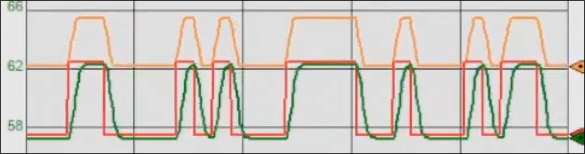
\includegraphics[width=0.7\textwidth]{img/prbs.png}
  \end{center}
  \caption{}\label{prbs}
\end{figure}

\subsection{Control con Horizonte Extendido}
\subsection{Implementación de control predictivo en planta de 4 estanques}
